% PCFPG paper skeleton (IEEEtran, conference). Compile on Overleaf: main.tex + refs.bib. Red [TODO] = fill from logs/bench.json.
\documentclass[conference]{IEEEtran}
\usepackage{cite}
\usepackage{amsmath,amssymb}
\usepackage{graphicx}
\usepackage{booktabs}
\usepackage{xcolor}
\usepackage{tikz}
\usetikzlibrary{arrows.meta,positioning,shapes.geometric}
\newcommand{\todo}[1]{\textcolor{red}{\textbf{[#1]}}}
\newcommand{\iou}{\mathrm{IoU}}
\newcommand{\resRoomIoU}{\todo{x}}\newcommand{\resRoomIoULo}{\todo{lo}}\newcommand{\resRoomIoUHi}{\todo{hi}}\newcommand{\resN}{\todo{n}}\newcommand{\resBaseIoU}{\todo{x}}\newcommand{\resK}{\todo{K}}
\InputIfFileExists{results_numbers.tex}{}{}
\begin{document}

\title{PCFPG: Parameter-Conditioned Residential Floor Plan Generation from Boundary and Room-Graph Specifications}
\author{\IEEEauthorblockN{\todo{Author name(s)}}
\IEEEauthorblockA{\todo{Department, Institution, City, Country}\\ \todo{email}}}
\maketitle

\begin{abstract}
We present PCFPG, a two-stage system that generates residential floor plans from a building boundary, typed rooms, a room-connectivity graph, an entrance and optional relative room sizes. A graph transformer (BoxNet) with per-room adaptive layer-norm conditioning proposes one rectangle per room; a U-Net (RefineNet) turns the rectangles into room regions; a rule-based builder produces right-angled rooms, walls, doors and windows; and a learned scorer selects the best of $K$ candidate layouts. Trained and evaluated on the ResPlan dataset ($n=\resN$ test plans), the system reaches a room IoU of \resRoomIoU{} (95\% CI [\resRoomIoULo, \resRoomIoUHi]) with $K=\resK$ candidates and 0.598 with one, against \resBaseIoU{} for a nearest-neighbour retrieval baseline that is given the true room sizes (paired difference $+0.448$, $p<10^{-3}$). It realises 98.3\% of requested doors and 93.7\% of requested adjacencies and follows requested relative room sizes to within 1.4--1.9 percentage points of total area. Ablations show that multi-hypothesis training lowers single-sample IoU but raises best-of-$K$ IoU, that the tiling loss helps slightly, and that test-time augmentation gives no measurable gain. Because connectivity and wall straightness are partly guaranteed by a rule-based builder---only 16\% of generated layouts, and 18\% of real layouts passed through the same builder, need no automatic repair---these metrics must be interpreted with care. We do not compare numerically with retrained published methods.
\end{abstract}

\begin{IEEEkeywords}
floor plan generation, graph-conditioned generation, transformers, ResPlan, layout synthesis
\end{IEEEkeywords}

\section{Introduction}
Automated floor-plan generation supports early-stage residential design by turning requirements---boundary, rooms, adjacencies, sizes---into candidate layouts. Prior work generates plans from layout graphs by retrieval and regression~\cite{hu2020graph2plan}, adversarial refinement~\cite{nauata2020housegan,nauata2021housegan++} or diffusion~\cite{shabani2023housediffusion}, mostly on the RPLAN data~\cite{wu2019rplan}. The recent ResPlan dataset~\cite{abouagour2025resplan} offers 17{,}000 vector-graph plans with richer structure.

We build a practical, end-to-end system on ResPlan and make the following contributions:
\begin{itemize}
\item a two-stage architecture combining a graph transformer for box placement with a U-Net for region refinement, conditioned on room type, entrance and relative size via adaptive layer-norm;
\item multi-hypothesis (winner-takes-all) training so that different noise samples yield distinct, individually plausible layouts;
\item a deterministic geometric builder producing orthogonal rooms, walls, doors and windows, plus a learned best-of-$K$ selector;
\item an open implementation with an interactive graph editor and 3D viewer, and an evaluation with bootstrap confidence intervals.
\end{itemize}
We do not claim superiority over published methods: the ResPlan paper reports no baseline results in the version we consulted, and other methods report different data and metrics.

\section{Related Work}
\textbf{Floor-plan generation.} RPLAN~\cite{wu2019rplan} introduced a large residential dataset and a data-driven pipeline. Graph2Plan~\cite{hu2020graph2plan} retrieves and adjusts layouts from a layout graph. House-GAN and House-GAN++~\cite{nauata2020housegan,nauata2021housegan++} use relational GANs with iterative refinement; HouseDiffusion~\cite{shabani2023housediffusion} denoises vector coordinates. ResPlan~\cite{abouagour2025resplan} proposes benchmark tasks (including constrained generation) and metrics such as IoU, room-count/type match, graph edit distance and FID.

\textbf{Building blocks.} We use transformers~\cite{vaswani2017attention} with adaptive layer-norm conditioning~\cite{peebles2023dit,perez2018film}, a U-Net~\cite{ronneberger2015unet}, GIoU~\cite{rezatofighi2019giou}, Hungarian matching~\cite{kuhn1955hungarian}, Weisfeiler--Lehman colours~\cite{shervashidze2011wl}, multiple-choice learning~\cite{guzman2012mcl}, total-variation regularisation~\cite{rudin1992tv} and Douglas--Peucker simplification~\cite{douglas1973peucker}.

\section{Data and Representation}
\textbf{Dataset.} ResPlan contains 17{,}000 plans as geometries per room type, walls, doors, windows, front door and footprint. Its primary room classes are bedroom, bathroom, kitchen and living, and secondary classes are balcony, storage, parking, pool and stair; there is no dining class. We use seven types: living, bedroom, bathroom, kitchen, balcony, storage, stair. We use the official split (train 13{,}053, validation 1{,}632, test 1{,}632) and keep plans with at most $M=16$ rooms, which covers 99.6\% of plans.

\textbf{Tensors.} Each plan is rasterised on a $128\times128$ canvas: boundary and front-door masks $c\in\{0,1\}^{2\times128\times128}$, room types $t\in\{0..6\}^{M}$ (padded), entrance flags, an edge matrix $E\in\{0,1,2\}^{M\times M}$ (none, adjacent, door), relative sizes $s\in\Delta^{M}$, boxes $b\in[0,1]^{M\times4}$ and a dense instance map. Rooms that are indistinguishable by type and graph neighbourhood share a Weisfeiler--Lehman colour, which defines groups within which predictions may be permuted.

\section{Method}
\begin{figure}[t]
\centering
\resizebox{\columnwidth}{!}{%
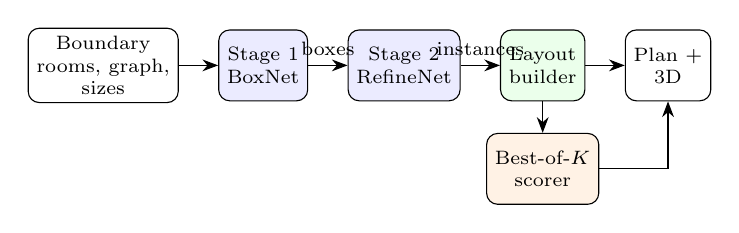
\begin{tikzpicture}[node distance=5mm, every node/.style={font=\scriptsize}, box/.style={draw,rounded corners,align=center,minimum height=9mm,inner sep=3pt}, arr/.style={-{Stealth[length=2mm]}}]
\node[box] (in) {Boundary\\ rooms, graph,\\ sizes};
\node[box,right=of in,fill=blue!8] (bn) {Stage 1\\ BoxNet};
\node[box,right=of bn,fill=blue!8] (rn) {Stage 2\\ RefineNet};
\node[box,right=of rn,fill=green!8] (lb) {Layout\\ builder};
\node[box,right=of lb] (out) {Plan +\\ 3D};
\draw[arr] (in)--(bn); \draw[arr] (bn)--node[above]{boxes}(rn); \draw[arr] (rn)--node[above]{instances}(lb); \draw[arr] (lb)--(out);
\node[box,below=4mm of lb,fill=orange!10] (sel) {Best-of-$K$\\ scorer};
\draw[arr] (lb)--(sel); \draw[arr] (sel.east)-|(out.south);
\end{tikzpicture}}
\caption{PCFPG pipeline. Stages 1--2 are learned; the builder is deterministic; $K$ candidates are generated and ranked.}
\label{fig:pipe}
\end{figure}

\subsection{Stage 1: BoxNet}
A CNN encodes the boundary (with coordinate channels) into a $16\times16$ grid of tokens. Each room is a token built from its type, entrance flag, noise vector $z$, and optionally its relative size and a ``size known'' flag. Four transformer layers (width 192, 6 heads) apply (i) self-attention among rooms with a learned per-head bias for each edge type, (ii) cross-attention to the boundary tokens and (iii) a feed-forward block; each sub-layer is modulated by adaptive layer-norm with zero-initialised gates driven by a per-room conditioning vector~\cite{peebles2023dit}. Deep supervision is applied to intermediate layers.

Predictions are matched to ground truth by the Hungarian algorithm~\cite{kuhn1955hungarian} restricted to Weisfeiler--Lehman-equivalent groups $\pi$:
\begin{equation}
\mathcal{L}_{\text{box}}=\sum_{r}\Big(5\,\lVert b_r-b^{*}_{\pi(r)}\rVert_1+2\big(1-\mathrm{GIoU}(b_r,b^{*}_{\pi(r)})\big)\Big).
\end{equation}
Two auxiliary terms are added: an adjacency hinge that penalises the gap between boxes of connected rooms (weight 8), and a ground-truth-anchored tiling loss on coverage, containment and stacking (weight 1). A pairwise box-overlap repulsion was measured to be uninformative on ResPlan (wrong layouts overlapped less than real ones) and is disabled. With $H=4$ noise samples per input, we use multiple-choice learning~\cite{guzman2012mcl}:
\begin{equation}
\mathcal{L}=0.9\min_{h}\mathcal{L}^{(h)}+0.1\,\tfrac1H\sum_{h}\mathcal{L}^{(h)}.
\end{equation}
Training uses a curriculum (size-noise $\sigma$ rising from 0 to 0.25, probability of known sizes falling from 0.9 to 0.6), random rotations/flips, AdamW~\cite{loshchilov2019adamw} and a one-cycle schedule~\cite{smith2019onecycle}.

\subsection{Stage 2: RefineNet}
A U-Net~\cite{ronneberger2015unet} receives 25 channels (boundary, front door, $16$ per-slot box masks, $7$ room-type masks) and outputs $17$ logits (outside plus one per slot), i.e.\ an instance segmentation. The loss is an edge-weighted cross-entropy plus an anisotropic total variation~\cite{rudin1992tv} that favours axis-parallel borders:
\begin{equation}
\mathcal{L}_{\text{ref}}=\frac{\sum_p w_p\,\mathrm{CE}(\hat y_p,y_p)}{\sum_p w_p}+3\,\mathrm{TV}_{\text{aniso}},
\end{equation}
where $w_p$ is increased on pixels adjacent to room borders. Training uses ground-truth boxes with jitter and soft edges, exponential-moving-average weights, and a final fine-tuning phase on BoxNet's own predicted boxes.

\subsection{Geometric layout builder}
Without learning, the builder (1) keeps the largest connected component per room and fills gaps, (2) simplifies room contours with Douglas--Peucker~\cite{douglas1973peucker} into strictly orthogonal polygons with coordinate clustering, (3) re-inserts rooms dropped by the network from the predicted boxes, (4) places walls on all inter-room borders, (5) cuts a door opening for every requested door edge and adds doors where needed so every room is reachable, (6) opens the entrance on an exterior wall and (7) adds windows to exterior walls of living rooms, bedrooms, bathrooms and kitchens. \emph{Because steps (3)--(5) repair outputs, completeness and connectivity are partly satisfied by construction; we therefore report pre- and post-repair rates where possible.}

\subsection{Candidate generation and selection}
For each input, $K$ noise seeds yield $K$ candidates; RefineNet logits are averaged over four flip/rotation transforms (test-time augmentation). Each candidate is described by ten features $f_k$ (door ratio, rooms present, connectivity, straightness, box consistency, box overlap, bad aspect ratios, size error, automatic-door count, rectangularity) and ranked by $\mathrm{score}(\ell)=\sum_k\lambda_k f_k(\ell)$, with $\lambda$ fitted by within-plan ridge regression to the candidate's true room IoU on validation plans.

\section{Experimental Setup}
\textbf{Training.} BoxNet: 200 epochs (about 53\,s per epoch), AdamW with a one-cycle schedule, batch 128, learning rate $6\times10^{-4}$ \todo{confirm these defaults were used}; RefineNet: \todo{epochs, batch, lr, fine-tuning}; ablation variants use the same budget and a single training run each; hardware: NVIDIA GeForce RTX 5050 Laptop GPU \todo{RAM}; framework: PyTorch~\cite{paszke2019pytorch}.

\textbf{Protocol.} All results use the ResPlan test split as present in our processed cache ($n=\resN$ plans; the official split lists 1{,}632 \todo{state why two plans are absent, e.g.\ preprocessing filters}). Each plan is regenerated from its own boundary, room types, entrance and connectivity graph. Two requested-size scenarios are used: \emph{default} (type-median relative sizes, what a user gets without specifying areas) and \emph{true} (the plan's actual relative sizes, which tests parameter conditioning). For each input, $K=\resK$ candidates are generated and the one with the highest learned score is returned (the scorer never sees the ground truth); ``$K{=}1$'' is a single sample. Values are averaged over the sampling seeds per plan; confidence intervals are percentile bootstrap intervals over plans (2{,}000 resamples)~\cite{efron1979bootstrap}; paired comparisons use the Wilcoxon signed-rank test with Holm correction and the Vargha--Delaney $A_{12}$ effect size.

\textbf{Metrics.} \emph{Fidelity to the reference layout}: matched room IoU, $\frac1{R}\sum_{r}\frac{|P_r\cap G_r|}{|P_r\cup G_r|}$, where rooms that are indistinguishable to the model (same Weisfeiler--Lehman colour) may be swapped by Hungarian matching~\cite{kuhn1955hungarian,shervashidze2011wl}; Stage-1 box IoU analogously. Because many layouts are valid for one specification, IoU measures agreement with one architect's choice, not quality. \emph{Constraint satisfaction}: adjacency recall $|E_{\mathrm{req}}\cap E_{\mathrm{real}}|/|E_{\mathrm{req}}|$ and precision $|E_{\mathrm{req}}\cap E_{\mathrm{real}}|/|E_{\mathrm{real}}|$ (two rooms are adjacent if they share at least 4\,px of border); door-graph distance $1-|E^{\mathrm{door}}_{\mathrm{req}}\cap E^{\mathrm{door}}_{\mathrm{real}}|/|E^{\mathrm{door}}_{\mathrm{req}}\cup E^{\mathrm{door}}_{\mathrm{real}}|$ (node identities are known, so graph edit distance reduces to this; it is \emph{not} comparable to published GED values); size error $\frac1R\sum_r|\hat s_r-s_r|$ between realised and requested area fractions, and their Spearman correlation. \emph{Validity}: a layout is valid after repair if all rooms are present as single connected regions and every room is reachable through doors; it is valid before repair if, using only the networks and geometry, all rooms are present, every requested door is placed and no door had to be added automatically. Footprint coverage and the fraction of room area outside the footprint are reported. \emph{Diversity}: mean pairwise $1-$matched IoU among the $K$ candidates of one input. \emph{Novelty}: nearest-neighbour IoU of the room-type map to training plans with the same room set (lower values indicate less copying; differing boundaries also lower it). \emph{Efficiency}: parameters, latency (p50/p95) and peak GPU memory.

\textbf{Baselines and references.} B0: mean box per room type (no learning). B1: retrieval of the nearest training plan with the same room-type multiset and most similar footprint, rooms assigned by type and size rank, clipped to the footprint (the retrieval stage of Graph2Plan~\cite{hu2020graph2plan} without its adjustment network; it ignores the graph but is given the true sizes). GT: the real layouts passed through the same builder and metrics, giving the ceiling for constraint metrics. Ablations remove one component at a time and retrain BoxNet with the same budget.

\textbf{Published methods.} Graph2Plan, House-GAN++ and HouseDiffusion~\cite{hu2020graph2plan,nauata2021housegan++,shabani2023housediffusion} were designed for other data and report other metrics; the ResPlan paper~\cite{abouagour2025resplan} gives no baseline results. We therefore do \emph{not} compare numerically with them. A fair comparison requires retraining each method on the ResPlan training split and evaluating on the same test plans with the same metrics.

\section{Results}
\IfFileExists{results_tables.tex}{\input{results_tables.tex}}{%
\todo{Run bench\_full.py, baselines.py and make\_tables.py, then place results\_tables.tex next to main.tex. Tables for main results, conditioning, baselines, efficiency and ablations appear here.}\label{tab:main}\label{tab:cond}\label{tab:base}\label{tab:eff}\label{tab:abl}}
\subsection{Main results}
Table~\ref{tab:main}: selecting the best of $K=8$ candidates raises room IoU from 0.598 [0.587, 0.609] to 0.672 [0.661, 0.682] and Stage-1 box IoU from 0.586 to 0.657 (non-overlapping intervals). Constraint metrics are high: 98.3\% of requested doors are realised, adjacency recall is 0.937 and precision 0.990, and 94.8\% of layouts are valid after repair, close to the 95.3\% of real layouts passed through the same builder (overlapping intervals).
Three caveats apply. (i) On door realisation (0.983 vs.\ 0.969) and adjacency recall (0.937 vs.\ 0.861) the system exceeds the ground-truth reference. The training losses and the selector explicitly reward these properties, so this indicates closer satisfaction of the specification, not better design than the real plans. (ii) Before repair only 16.0\% of layouts are valid (GT reference 17.5\%): about 84\% of generated plans, and about 82\% of real plans passed through the same builder, require at least one automatically added door or restored room. The builder's repairs are therefore routine, and connectivity or completeness should not be read as evidence about the networks alone. (iii) Footprint coverage is 1.0 by construction, and the 8\% of room area outside the footprint is an artefact of instance maps extending into wall thickness that also occurs in the real plans (8.9\%).

\subsection{Parameter conditioning}
Table~\ref{tab:cond}: the realised room sizes follow the requested relative sizes closely, with a mean absolute deviation of 1.4 percentage points of total area when the plan's true sizes are requested and 1.9 with type-median sizes (Spearman $\rho$ 0.925 and 0.901). Requesting the true sizes raises room IoU from 0.672 to 0.698, so size information helps reproduce the reference layout. The mean relative size error is similar in both settings (0.200 vs.\ 0.185) and has a wide interval for true sizes because small rooms dominate relative errors. Adjacency recall is essentially unchanged (0.940 vs.\ 0.937).

\subsection{Comparison with baselines}
Table~\ref{tab:base}: with true sizes requested, our best-of-$K$ room IoU is 0.698 against 0.250 for retrieval (B1), a paired difference of $+0.448$ [0.435, 0.462] (Holm-corrected Wilcoxon $p<10^{-3}$, $A_{12}=0.89$); adjacency recall is higher by 0.329 and the size error is lower by 0.017 (ours smaller in about 87\% of pairs). The mean-box baseline reaches a box IoU of 0.086 against 0.685. B1 is deliberately simple: it ignores the graph and cannot reshape a retrieved layout to the footprint, so part of the gap reflects boundary mismatch. It is not a published method and says nothing about Graph2Plan or other published systems.

\subsection{Ablations}
Table~\ref{tab:abl} (one training run per variant, same budget; $p$-values are paired Wilcoxon tests over test plans and do not capture training-run variance). \emph{Multi-hypothesis training} matters most: without it, best-of-8 room IoU falls from 0.672 to 0.638 ($+0.033$ for the full model, $p<10^{-3}$), yet single-sample ($K{=}1$) IoU is \emph{higher} (0.633 vs.\ 0.598). Without it, eight candidates barely help (0.633 to 0.638), whereas with it they add 0.074; the technique thus trades single-sample accuracy for useful diversity. The \emph{tiling loss} gives a small gain (0.662 to 0.672, $+0.010$, $p=7\times10^{-4}$, which stays below 0.05 after a Bonferroni correction over four planned ablations), but with a single run per variant a one-point difference cannot be separated from run-to-run variation. \emph{Test-time augmentation} brings no measurable benefit in room IoU ($+0.000$, $p=0.99$) although it multiplies the refinement cost; we did not time the model without it. \todo{Adjacency-loss ablation: add once its evaluation is available; do not interpret before then.}

\subsection{Diversity, novelty and efficiency}
Table~\ref{tab:eff}: the eight candidates for one input differ substantially (mean pairwise $1-$IoU of 0.299). The nearest-neighbour type-map IoU to training plans with the same room set is 0.490 on average, which suggests that outputs are not, on average, near-copies of training layouts; boundary differences lower this value and we did not measure the near-copy rate. The models have 10.20\,M (BoxNet) and 7.77\,M (RefineNet) parameters; latency per plan including geometric post-processing is 0.13\,s ($K{=}1$) and 0.61\,s ($K{=}8$) at the median, with a peak GPU memory of 278\,MB (30 test plans timed).


\IfFileExists{fig_qualitative.png}{\begin{figure*}[t]\centering\includegraphics[width=0.8\textwidth]{fig_qualitative.png}\caption{Randomly selected test plans (not cherry-picked): input, ground truth, retrieval baseline B1 and our best-of-$K$ layout with walls, doors and windows.}\label{fig:qual}\end{figure*}}{\todo{Figure: run make\_figures.py and place fig\_qualitative.png next to main.tex.}}
\IfFileExists{fig_candidates.png}{\begin{figure}[t]\centering\includegraphics[width=\columnwidth]{fig_candidates.png}\caption{Different candidates for one input (score $s$); the best-scoring one is returned.}\label{fig:cand}\end{figure}}{}

\section{Discussion and Limitations}
Stage~1 box placement remains the accuracy bottleneck: the final room IoU (0.672) is well below the 0.917 that RefineNet reaches when given the real boxes (\texttt{evaluate.py}, 100 test plans, measured before the geometric builder and therefore only indicative of the Stage-2 ceiling). IoU against a single reference layout understates quality because many layouts are valid for one specification, which is why constraint satisfaction is reported alongside it. Metrics that the selector or the builder optimise directly (door realisation, connectivity, adjacency) are inflated by that optimisation and by automatic repairs; the GT reference column and the before-repair rows are included to make this visible. A better selector could recover part of the remaining gap: the oracle best-of-8 box IoU is 0.710 against 0.657 for learned selection, although these come from different evaluation sets (100 and 1{,}630 plans) and are indicative only. Further limits: one trained model per configuration (the seeds are sampling seeds, not independent training runs), a single run per ablation, no distribution metrics (FID, graph edit distance) and no human evaluation, no numerical comparison with retrained published methods, at most 16 rooms, seven room types, single-storey plans, and furniture and stairs in the 3D viewer that are illustrative and not predicted.

\section{Conclusion}
PCFPG combines graph-conditioned box prediction, region refinement and geometric construction to produce editable, three-dimensional floor plans from ResPlan. On 1{,}630 test plans it reaches a room IoU of 0.672 with eight candidates, follows the requested connectivity and relative sizes closely, and clearly outperforms a retrieval baseline, while multi-hypothesis training proves to be the key ingredient for useful candidate diversity. Future work includes fair comparisons with retrained baselines on the shared ResPlan split, constraint-satisfaction and diversity metrics, and multi-seed statistics.

\bibliographystyle{IEEEtran}
\bibliography{refs}
\end{document}